% ---------
% --------
%!TEX TS-program = pdflatex
%!TEX encoding = UTF-8 Unicode
%!TEX spellcheck = English (Aspell)

\documentclass[11pt]{article}
\usepackage{lucy,handout,graphicx}
\usepackage{tikz,chessfss}
\usepackage{fourier-orns}
\usepackage{mathtools}
\usepackage[normalem]{ulem} % either use this (simple) or
\pagestyle{empty}

\allowdisplaybreaks

\begin{document}


\begin{center}
\Large\textbf{CSCI 332, Fall 2026}%
\\
\LARGE\textbf{In-class Activity}%
\end{center}

In the $N$ queens problem, your goal is to find a placement of $N$
queens on an $N$-by-$N$ chessboard so that no two queens can attack one another.

\begin{enumerate}
\item
Is the following a valid placement of 4 queens
on a 4x4 chessboard? Why or why not?

\begin{center}
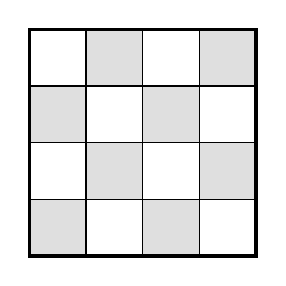
\begin{tikzpicture}[x=0.72cm,y=0.72cm]
   \foreach \x in {0,...,3} {
      \foreach \y in {0,...,3} {
         \pgfmathtruncatemacro{\shade}{mod(\x+\y,2)}
         \ifnum\shade=0
            \fill[gray!25] (\x,\y) rectangle ++(1,1);
         \fi
      }
   }
   \draw[step=1,line width=0.5pt] (0,0) grid (4,4);
   \draw[line width=1.2pt] (0,0) rectangle (4,4);
   \foreach \x/\y in {0/3,1/0,2/2,3/1} {
      \node at ({\x+0.5},{\y+0.5}) {\fontsize{18}{18}\selectfont\symqueen};
   }
\end{tikzpicture}
\end{center}

\item Draw all valid placements for $N=4$. (you may not need every board)

% todo: make 4 empty chessboards for them to fill in, all in a horizontal line

\begin{center}
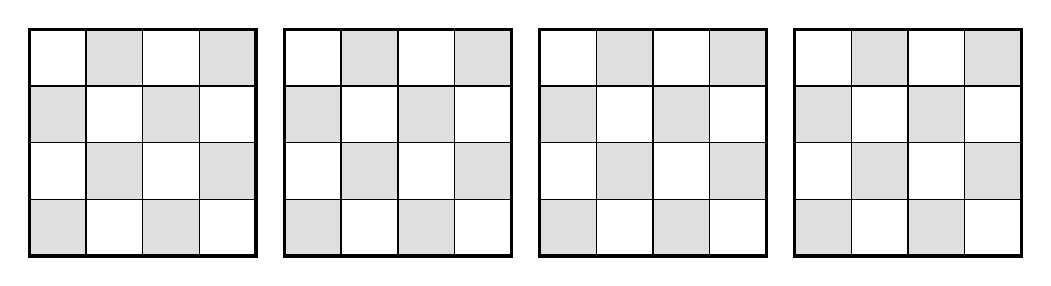
\begin{tikzpicture}[x=0.72cm,y=0.72cm]
   \foreach \offset in {0,4.5,9,13.5} {
      \begin{scope}[shift={(\offset,0)}]
         \foreach \x in {0,...,3} {
            \foreach \y in {0,...,3} {
               \pgfmathtruncatemacro{\shade}{mod(\x+\y,2)}
               \ifnum\shade=0
                  \fill[gray!25] (\x,\y) rectangle ++(1,1);
               \fi
            }
         }
         \draw[step=1,line width=0.5pt] (0,0) grid (4,4);
         \draw[line width=1.2pt] (0,0) rectangle (4,4);
      \end{scope}
   }
\end{tikzpicture}
\end{center}

\item What properties do you notice about valid placements?

\vspace{1in}

\item Try to use those to come up with an algorithm to enumerate all possible
valid placements for any $N$. (Ideally, a recursive algorithm!)

\end{enumerate}

%%%%%%%%%%%%%%%%%%%%
\end{document}
